%!TEX TS-program = pdflatexmk
\documentclass[]{asme2ej}

%\usepackage{epsfig} %% for loading postscript figures
\usepackage{graphicx}
\graphicspath{ {images/} }

\usepackage{amsmath,amssymb}
\usepackage{hyperref}
\usepackage[]{natbib}

\newcommand{\reffig}[1]{Fig.~\ref{#1}}

\title{Exoplanet Direct Imaging Mission Simulation Code Interface Control Document}

%%% first author
\author{Daniel Garrett and Dmitry Savransky
    \affiliation{
	Sibley School of Mechanical and Aerospace Egnineering\\
	Cornell University\\
	Ithaca, NY 14853\\
    }	
}


\begin{document}

\maketitle    

%%%%%%%%%%%%%%%%%%%%%%%%%%%%%%%%%%%%%%%%%%%%%%%%%%%%%%%%%%%%%%%%%%%%%%
\begin{abstract}
{\it 
This document describes the required input/output interfaces between each stand-alone module in the exoplanet direct imaging mission simulation code.
}
\end{abstract}

\tableofcontents

%%%%%%%%%%%%%%%%%%%%%%%%%%%%%%%%%%%%%%%%%%%%%%%%%%%%%%%%%%%%%%%%%%%%%%
\begin{nomenclature}
\entry{HE}{Heliocentric Equatorial}
\entry{ICD}{Interface Control Document}
\entry{MJD}{Modified Julian Day}
\entry{OD}{Observatory Definition}
\entry{OSD}{Optical System Description}
\entry{PP}{Post-Processing}
\entry{PPD}{Planet Population Definition}
\entry{PPM}{Planet Physical Model}
\entry{SC}{Star Catalog}
\entry{SE}{Survey Ensemble}
\entry{SS}{Survey Simulation}
\entry{SU}{Simulated Universe}
\entry{TL}{Target List}
\end{nomenclature}

%%%%%%%%%%%%%%%%%%%%%%%%%%%%%%%%%%%%%%%%%%%%%%%%%%%%%%%%%%%%%%%%%%%%%%
% INTRODUCTION
%%%%%%%%%%%%%%%%%%%%%%%%%%%%%%%%%%%%%%%%%%%%%%%%%%%%%%%%%%%%%%%%%%%%%%

\section{Introduction}

The exoplanet direct imaging simulation code generates ensembles of mission simulations for exoplanet direct imaging missions to estimate science yields. The code consists of stand-alone modules written in Python which may be modified without requiring modifications to other portions of the code. This allows the code to be easily used to investigate new designs for exoplanet direct imaging missions. This document describes the required input/output interfaces for the stand-alone modules to enable this flexibility.

\subsection{Purpose}
This Interface Control Document (ICD) describes the interface between modules of the code. The data inputs and outputs of each module are described. Following these guidelines will allow the code to be updated to accommodate new mission designs.

\subsection{Scope}
This ICD defines the interfaces between modules of the code. It does not specify the contents of the individual modules beyond a general description of what each module does.

\subsection{Glossary}
This section will contain definition of terms used throughout the document if needed.

%%%%%%%%%%%%%%%%%%%%%%%%%%%%%%%%%%%%%%%%%%%%%%%%%%%%%%%%%%%%%%%%%%%%%%%%%%
% OVERVIEW
%%%%%%%%%%%%%%%%%%%%%%%%%%%%%%%%%%%%%%%%%%%%%%%%%%%%%%%%%%%%%%%%%%%%%%%%%%

\section{Overview}
The code framework consists of stand-alone modules. The fundamental inputs of the simulation may require external data. These include the Optical System Description (OSD), Star Catalog (SC), Planet Population Definition (PPD), Planet Physical Model (PPM), Observatory Definition (OD), Rules, and Post-Processing (PP) modules. The other modules used in mission simulation require a combination of the fundamental inputs as well as modules upstream in \reffig{fig:codeflow}. These include Target List (TL), Simulated Universe (SU), Survey Simulation (SS), and Survey Ensemble (SE) modules.

%\begin{figure}[t]
%    \centering
%    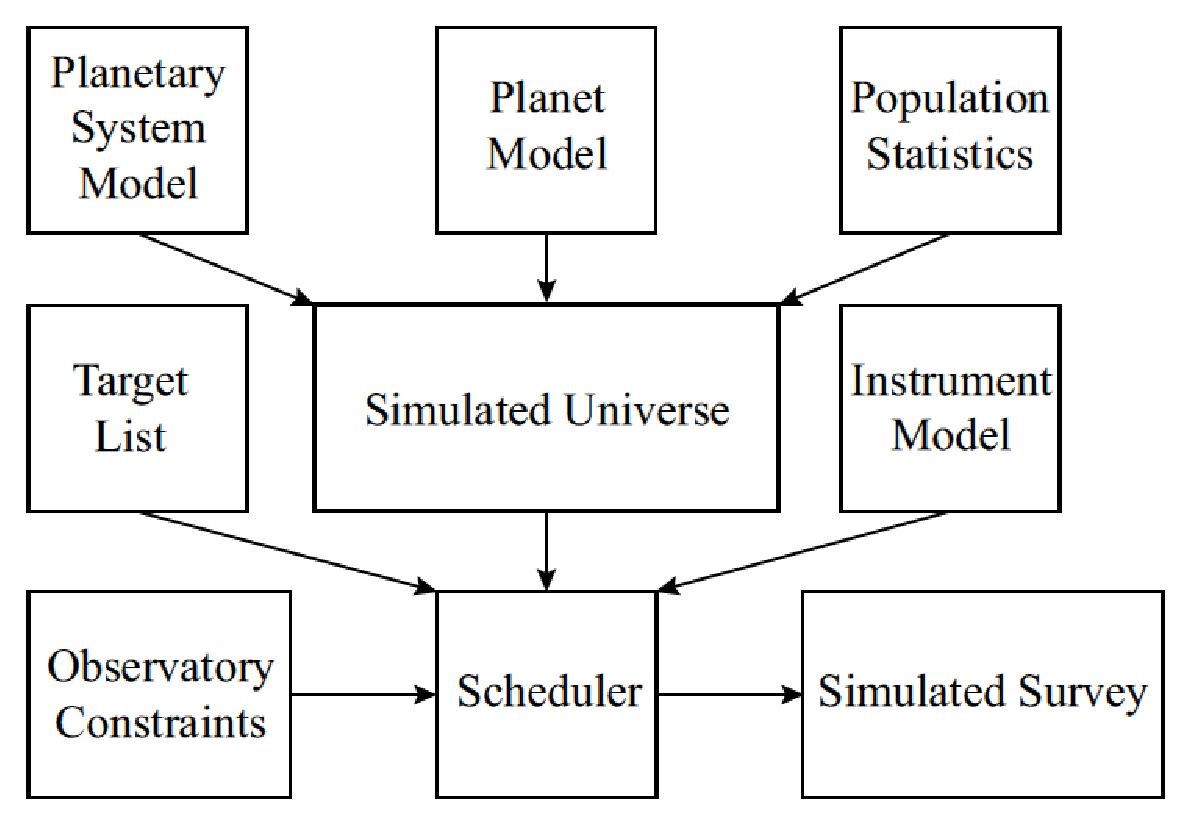
\includegraphics[width=5in]{Framework}
%    \caption{Exoplanet direct imaging simulation code framework}
%    \label{figure_framework}
%\end{figure}

\reffig{fig:codeflow} shows the relationships of the component software modules classified as either input modules or simulation modules. The input modules contain specific mission design parameters. The simulation modules take the information contained in the input modules and perform mission simulation tasks.  Any module may perform any number or kind of calculations using any or all of the input parameters provided.  They are only constrained by their input and output specification, which is designed to be as flexible as possible, while limiting unnecessary data passing to speed up execution.

\begin{figure}[ht]
    \begin{center}
        \begin{tabular}{c}
            \includegraphics[width=\textwidth]{codeflow2}
        \end{tabular}
   \end{center}
   \caption 
   { \label{fig:codeflow} Flowchart of mission simulation. Each box represents a component software module which interacts with other modules as indicated by the arrows. The simulation modules (those that are not classified as input modules) pass all input modules along with their own output.  Thus, the Survey Ensemble module has access to all of the input modules and all of the upstream simulation modules.} 
\end{figure} 


%%%%%%%%%%%%%%%%%%%%%%%%%%%%%%%%%%%%%%%%%%%%%%%%%%%%%%%%%%%%%%%%%%%%%%%%%
% GLOBAL SPECIFICATIONS
%%%%%%%%%%%%%%%%%%%%%%%%%%%%%%%%%%%%%%%%%%%%%%%%%%%%%%%%%%%%%%%%%%%%%%%%%

\section{Global Specifications}
This section specifies important information shared throughout the code.
\begin{description}
    \item[Common Epoch] \hfill \\ J2000
    \item[Common Reference Frame] \hfill \\ Heliocentric Equatorial (HE)
    \item[Common Time] \hfill \\ Modified Julian Day (MJD $\triangleq$ JD - 2400000.5)
\end{description}

\subsection{Python Packages}
The following Python packages are used for the WFIRST-specific version of exoplanet mission simulation:

\begin{itemize}
    \item astropy
        \begin{itemize}
            \item astropy.time
            \item astropy.units
        \end{itemize}
    \item numpy 
\end{itemize}

%%%%%%%%%%%%%%%%%%%%%%%%%%%%%%%%%%%%%%%%%%%%%%%%%%%%%%%%%%%%%%%%%%%%
% BACKBONE
%%%%%%%%%%%%%%%%%%%%%%%%%%%%%%%%%%%%%%%%%%%%%%%%%%%%%%%%%%%%%%%%%%%%

\section{Backbone}
All simulation execution will be performed by the backbone.  This set of functions will have very limited built-in functionality, and will primarily be tasked with parsing the input specification described below, and then calling the specified instances of each of the framework modules, detailed in \S\ref{sec:modules}.

A simulation specification is a single JSON-formatted (\url{http://json.org/}) file that encodes user-settable parameters and module names.  The backbone will contain a reference specification with \emph{all} parameters and modules set.  In the initial parsing of the user-supplied specification, it will be merged with the reference specification such that any fields not set by the user will be assigned to their reference (default) values. 

The backbone will contain a standalone specification parser that will check specification files for internal consistency.  For example, if modules carry mutual dependencies, the specification parser will return an error if these are not met for a given specification.  Similarly, if modules are selected with optional top level inputs, warnings will be generated if these are not set in the same specification files.

The backbone will contain an interactive function to help users generate specification files via a series of questions.

\subsection{Specification Format}
\begin{verbatim}
{
  "missionLifetime": 6,
  "missionDutyCycle": 0.24,
  "starlightSupressionSystems": [
    {
      "type": "SDO",
      "occulterDiameter": 50,
      "occulterDistance": 50000,
      "PSFfile": "/data/sdo1_psf.fits",
      "throughputFile": "/data/sdo1_thru.fits"
    },
    {
      "type": "coronagraph",
      "IWA": 3,
      "PSFfile": "/data/coron1_psf.fits",
      "throughputFile": "/data/coron1_thru.fits"
    }
  ],
  OSDmod: "hybridOSD1"
}
\end{verbatim}

%%%%%%%%%%%%%%%%%%%%%%%%%%%%%%%%%%%%%%%%%%%%%%%%%%%%%%%%%%%%%%%%%%%%%%%%%
% FUNDAMENTAL INPUT MODULE DESCRIPTION
%%%%%%%%%%%%%%%%%%%%%%%%%%%%%%%%%%%%%%%%%%%%%%%%%%%%%%%%%%%%%%%%%%%%%%%%%

\section{Modules of Fundamental Inputs}\label{sec:modules}
Modules containing fundamental inputs include Optical System Description (OSD), Star Catalog (SC), Planet Population Definition (PPD), Planet Physical Model (PPM), Observatory Definition (OD), Rules, and Post-Processing (PP). Much of the work of these modules will be reading external data and formatting the data for use by other modules. This section defines the input, output, and interface of each of these modules.

% OPTICAL SYSTEM DESCRIPTION NEEDS UPDATING

\subsection{Optical System Description (OSD) NEEDS UPDATING}
The Optical System Description module contains all of the necessary information to describe the effects of the telescope and starlight suppression system on the target star and planet wavefronts.  This requires encoding the design of both the telescope optics and the specific starlight suppression system, whether it be an internal coronagraph or an external occulter.  The encoding can be achieved by specifying Point Spread Functions (PSF) for on- and off-axis sources, along with (potentially angular separation-dependent) contrast and throughput definitions.  At the opposite level of complexity, the encoded portions of this module may be a description of all of the optical elements between the telescope aperture and the imaging detector, along with a method of propagating an input wavefront to the final image plane.  Intermediate implementations can include partial propagations, or collections of static PSFs representing the contributions of various system elements.  The encoding of the optical train will allow for the extraction of specific bulk parameters including the instrument inner working angle (IWA), outer working angle (OWA), and mean and max contrast and throughput.

If the starlight suppression system includes active wavefront control, i.e., via one or more deformable mirrors (DM)  \citep{cahoy2014wavefront}, then this module must also encode information about the sensing and control mechanisms.  Again, this can be achieved by simply encoding a static targeted DM shape, or by dynamically calculating DM settings for specific targets via simulated phase retrieval.  As wavefront control residuals may be a significant source of error in the final contrast budget, it is vitally important to include the effects of this part of the optical train.

The optical system description can optionally include stochastic wavefront-error generating components.  Again, there is a wide range of possible encodings and complexities.  They could be Gaussian errors on the contrast curves sampled during survey simulation to add a random element to the achieved contrast on each target.  Alternatively, in cases where an active wavefront control system is modeled, stochastic wavefront errors could be introduced by simulating the measurement noise on the wavefront sensor (either again as drawn from pre-determined distributions, or additively from various detector and astrophysical noise sources).  For external occulters, we draw on the large body of work on the effects of occulter shape and positioning errors on the achieved contrast, as in \citet{shaklan2010error}.

Finally, the optical system description must also include a description of the science instrument itself.  The baseline instrument is assumed to be an imaging spectrometer.  The encoding must provide the spatial and wavelength coverage of the instrument as well as sampling for each, along with detector details such as read noise, dark current, and readout cycle.  Optionally, this portion of the module may include descriptions of specific readout modes, i.e., in cases where Fowler sampling \citep{fowler1990demonstration} or other noise-reducing techniques are employed.

% STAR CATALOG

\subsection{Star Catalog (SC)}
The Star Catalog module includes detailed information about potential target stars drawn from general databases such as SIMBAD \citep{wenger2000simbad}, mission catalogs such as Hipparcos \citep{perryman1997hipparcos}, or from existing curated lists specifically designed for exoplanet imaging missions \citep{turnbull2012search}.  Information to be stored, or accessed by this module will include  target positions and proper motions at the reference epoch, catalog identifiers (for later cross-referencing), bolometric luminosities, stellar masses, and magnitudes in standard observing bands.  Where direct measurements of any value are not available, values are synthesized from ancillary data and empirical relationships, such as color relationships and mass-luminosity relations \citep{henry2004}.

This module will not provide any functionality for picking the specific targets to be observed in any one simulation, nor even for culling targets from the input lists where no observations of a planet could take place.  This is done in the Target List module as it requires interactions with the Planetary Population module (to determine the population of interest), the Optical System Description module (to define the capabilities of the instrument), and Observatory Definition module (to determine if the view of the target is unobstructed).

\subsubsection{Inputs}
\begin{description}
    \item[star catalog information] \hfill \\
    Information from an external star catalog containing the target stars
\end{description}

\subsubsection{Outputs} \label{starcatalog}
\begin{description}
    \item[missionsim.starcatalog.radeg] \hfill \\
    List of target star right ascension values in degrees
    \item[missionsim.starcatalog.decdeg] \hfill \\
    List of target star declination values in degrees
    \item[missionsim.starcatalog.pmra] \hfill \\
    List of target star right ascension proper motion values in mas/yr
    \item[missionsim.starcatalog.pmdec] \hfill \\
    List of target star declination proper motion values in mas/yr
    \item[missionsim.starcatalog.rv] \hfill \\
    List of target star radial velocities in km/s
    \item[missionsim.starcatalog.parx] \hfill \\
    List of target star parallax values in mas
\end{description}

% PLANET POPULATION DEFINITION NEEDS UPDATING

\subsection{Planet Population Definition (PPD) NEEDS UPDATING}
The Planet Population Description module encodes the density functions of all required planetary parameters, both physical and orbital. These include semi-major axis, eccentricity, orbital orientation, and planetary radius and mass. Certain parameter models may be empirically derived \citep{Savransky2011} while others may come from analyses \citep{Dressing2013,Fortney2007} of observational surveys such as the Keck Planet Search \citep{Cumming2008,Howard2010}, Kepler \citep{Batalha2013,Fressin2013,Petigura2013}, and ground-based imaging surveys including the Gemini Planet Imager Exoplanet Survey \citep{McBride2011,Macintosh2014}.  This module also encodes the limits on all parameters to be used for sampling the distributions and determining derived cutoff values such as the maximum target distance for a given instrument's IWA.

The Planet Population Description module does not model the physics of planetary orbits or the amount of light reflected or emitted by a given planet, but rather only encodes the statistics of planetary occurrence and properties.  As this encoding is based on density functions, it fully supports modeling `toy' universes where all parameters are fixed, in which case all of the distributions become delta functions.  We can equally use this encoding to generate simulated universes containing only `Earth-twins' to compare with previous studies as in \citet{brown2005} or \citet{Stark2014}.  Alternatively, the distributions can be selected to mirror, as closely as possible, the known distributions of planetary parameters.  As this knowledge is limited to specific orbital or mass/radius scales, this process invariably involves some extrapolation.

% PLANET PHYSICAL MODEL NEEDS UPDATING

\subsection{Planet Physical Model (PPM) NEEDS UPDATING}
The Planet Physical Model module contains models of the light emitted or reflected by planets in the wavelength bands under investigation by the current mission simulation.  It takes as inputs the physical quantities sampled from the distributions in the Planet Population module and generates synthetic spectra (or band photometry, as appropriate).  The specific implementation of this module can vary greatly, and can be based on any of the many available planetary albedo, spectra and phase curve models \citep{Pollack1986,Marley1999,Fortney2008,Cahoy2010,Spiegel2012,burrows1997nongray,burrows2003beyond}.

% TIME KEEPING WORK IN PROGRESS
\subsection{Time}
The Time module is responsible for keeping track of the current mission time.  It encodes only the mission start time, the mission duration, and the current time within a simulation.  All functions in all modules requiring knowledge of the current time call functions or access parameters implemented within the Time module.  Internal encoding of time is implemented as the time from mission start (measured in days).  The Time module also provides functionality for converting between this time measure and standard measures such as Julian Day Number and UTC time.

\subsubsection{Lifetime}

\subsubsection*{Inputs}
\begin{itemize}
    \item
    \begin{description}
        \item[start] \hfill \\
        Mission start time in MJD
        \item[finish] \hfill \\
        Mission end time in MJD
    \end{description}
\end{itemize}

\subsubsection*{Outputs}
\begin{itemize}
    \item
    \begin{description}
        \item[missionsim.time.start] \hfill \\
        Mission start time in MJD
        \item[missionsim.time.finish] \hfill \\
        Mission end time in MJD
    \end{description}
\end{itemize}

\subsubsection{Current Mission Time Update}

\subsubsection*{Inputs}
\begin{itemize}
    \item 
    \begin{description}
        \item[missionsim.time.currenttime] \hfill \\
        Current mission time in MJD (offset to zero at mission start)
        \item[Time Step] \hfill \\
        Time step in MJD to next mission time
    \end{description}
\end{itemize}

\subsubsection*{Outputs}
\begin{itemize}
    \item
    \begin{description}
        \item[missionsim.time.currenttime] \hfill \\
        Update the mission time
    \end{description}
\end{itemize}

% OBSERVATORY DEFINITION CURRENTLY WORKING

\subsection{Observatory Definition (OD) CURRENTLY WORKING}
The Observatory Definition module contains all of the information specific to the space-based observatory not included in the Optical System Description module. The module has three main tasks: orbit, duty cycle, and keepout definition, which are implemented as functions within the module. The inputs and outputs for these functions are represented schematically in \reffig{fig:observatory}.

\begin{figure}[ht]
    \begin{center}
        \begin{tabular}{c}
            \includegraphics[width=1\textwidth]{observatory2}
        \end{tabular}
   \end{center}
   \caption 
   { \label{fig:observatory} Depiction of Observatory Definition module including inputs, tasks, and outputs. } 
\end{figure} 

The observatory orbit plays a key role in determining which of the target stars may be observed for planet finding at a specific time during the mission lifetime. The Observatory Definition module's orbit function takes the current mission time as input and outputs the observatory's position vector. The position vector is standardized throughout the modules to be referenced to a heliocentric equatorial frame at the J2000 epoch. The observatory's position vector is used in the keepout definition task and Target List module to determine which of the stars from the Star Catalog may be targeted for observation at the current mission time.

The duty cycle determines when during the mission timeline the observatory is allowed to performing planet-finding operations. The duty cycle function takes the current mission time as input and outputs the next available time when exoplanet observations may begin or resume, along with the duration of the observational period. The outputs of this task are used in the Survey Simulation module to determine when and how long exoplanet finding and characterization observations occur.  The specific implementation of the duty cycle function can have significant effects on the science yield of the mission.  For example, if the observing program is pre-determined, such that exoplanet observations can only occur at specific times and last for specific durations, this significantly limits the observatory's ability to respond dynamically to simulated events, such as the discovery of an exoplanet candidate.  This can potentially represent a sub-optimal utilization of mission time, as it may prove to be more efficient to immediately spectrally characterize good planetary candidates rather than attempting to re-observe them at a later epoch.  It also limits the degree to which followup observations can be scheduled to match the predicted orbit of the planet.  Alternatively, the duty cycle function can be implemented to give the exoplanet observations the highest priority, such that all observations can be scheduled to attempt to maximize dynamic completeness \citep{brown2010new} or some other metric of interest. 

The keepout definition determines which target stars are observable at a specific time during the mission simulation and which are unobservable due to bright objects within the field of view such as the sun, moon, and solar system planets.  The keepout volume is determined by the specific design of the observatory and, in certain cases, by the starlight suppression system.  For example, in the case of external occulters, the sun cannot be within the 180$^\circ$ annulus immediately behind the telescope (with respect to the line of sight) as it would be reflected by the starshade into the telescope.  The  keepout definition function takes the current mission time and Star Catalog module output as inputs and outputs a list of the target stars which are observable at the current time. It constructs position vectors of the target stars and bright objects which may interfere with observations with respect to the observatory. These position vectors are used to determine if bright objects are in the field of view for each of the potential stars under exoplanet finding observation. If there are no bright objects obstructing the view of the target star, it becomes a candidate for observation in the Survey Simulation module.

In addition to these functions, the observatory definition can also encode finite resources that are used by the observatory throughout the mission.  The most important of these is the fuel used for stationkeeping and repointing, especially in the case of occulters which must move significant distances between observations.  We could also consider the use of other volatiles such as cryogens for cooled instruments, which tend to deplete solely as a function of mission time.  This module also allows for detailed investigations of the effects of orbital design on the science yield, e.g., comparing the baseline geosynchronous 28.5$^{\circ}$ inclined orbit for WFIRST-AFTA  \citep{Spergel2013} with an L2 halo orbit proposed for other exoplanet imaging mission concepts  \citep{savransky2010occulting}. 

\subsubsection{Orbit}

\subsubsection*{Inputs}
\begin{itemize}
    \item
    \begin{description}
        \item[Current Mission Time] \hfill \\
        Current mission time in MJD
    \end{description}
\end{itemize}

\subsubsection*{Outputs}
\begin{itemize}
    \item
    \begin{description}
        \item[missionsim.observatory.r\_sc] \hfill \\
        Observatory orbit position in HE reference frame at current mission time
    \end{description}
\end{itemize}

\subsubsection{Duty Cycle}

\subsubsection*{Inputs}
\begin{itemize}
    \item
    \begin{description}
        \item[Current Mission Time] \hfill \\
        Current mission time in MJD
    \end{description}
\end{itemize}

\subsubsection*{Outputs}
\begin{itemize}
    \item
    \begin{description}
        \item[missionsim.observatory.nexttime] \hfill \\
        Next available times in MJD
        \item[missionsim.observatory.nextduration] \hfill \\
        Time duration in MJD for next exoplanet detection and characterization referenced at \\ \texttt{missionsim.observatory.nexttime}
    \end{description}
\end{itemize}

\subsubsection{Keepout Definition}

\subsubsection*{Inputs}
\begin{itemize}
    \item
    \begin{description}
        \item[Current Mission Time] \hfill \\
        Current mission time in MJD 
        \item[missionsim.starcatalog] \hfill \\
        Output of SC module. See \ref{starcatalog} for definitions
    \end{description}
\end{itemize}

\subsubsection*{Outputs}
\begin{itemize}
    \item 
    \begin{description}
        \item[missionsim.observatory.ko] \hfill \\
        List of Boolean values for each target at current mission time where true is when a target is unobstructed in the keepout zone and false is when a target cannot be observed due to obstructions in the keepout zone
    \end{description}
\end{itemize}

% RULES NEEDS UPDATING

\subsection{Rules NEEDS UPDATING}
The Rules module contains additional constraints placed on the mission design not contained in other modules. These constraints are passed into the Survey Simulation module to control the simulation. For example, a constraint in the Rules module could include prioritization of revisits to stars with detected exoplanets for characterization when possible. This rule would force the Survey Simulation module to simulate observations for target stars with detected exoplanets when the Observatory Module determines those stars are observable.

The Rules module also encodes the calculation of integration time for an observation.  This can be based on achieving a pre-determined signal to noise (SNR) metric (with various possible definitions), or via a probabilistic description as in \citet{kasdin2006}.  This requires also defining a model for the background contribution due to all astronomical sources and especially due to zodiacal and exozodiacal light \citep{Stark2014}.

The integration time calculation can have significant effects on science yield---integrating to the same SNR on every target may represent a suboptimal use of mission time, as could integrating to achieve the minimum possible contrast on very dim targets.  Changing the implementation of the Rules module allows exploration of these tradeoffs directly.

% POST-PROCESSING NEEDS UPDATING

\subsection{Post-Processing (PP) NEEDS UPDATING}
The Post-Processing module encodes the effects of post-processing on the data gathered in a simulated observation, and the effects on the final contrast of the simulation.  In the simplest implementation, the Post-Processing module does nothing and simply assumes that the attained contrast is some constant value below the instrument's designed contrast--that post-processing has the effect of uniformly removing background noise by a pre-determined factor.  A more complete implementation actually models the specific effects of a selected post-processing technique such as LOCI  \citep{lafreniere2007new} or KLIP  \citep{soummer2012detection} on both the background and planet signal via either processing of simulated images consistent with an observation's parameters, or by some statistical description.

The Post-Processing module is also responsible for determining whether a planet detection has occurred for a given observation, returning one of four possible states---true positive (real detection), false positive (false alarm), true negative (no detection when no planet is present) and false negative (missed detection).  These can be generated based solely on statistical modeling as in \citet{kasdin2006}, or can again be generated by actually processing simulated images.

%%%%%%%%%%%%%%%%%%%%%%%%%%%%%%%%%%%%%%%%%%%%%%%%%%%%%%%%%%%%%%%%%%%%%%%%%
% Modules using fundamental inputs
%%%%%%%%%%%%%%%%%%%%%%%%%%%%%%%%%%%%%%%%%%%%%%%%%%%%%%%%%%%%%%%%%%%%%%%%%

\section{Modules Using Internally Generated Data}
Modules using data generated by the fundamental input modules include Target List (TL), Simulated Universe (SU), Survey Simulation (SS), and Survey Ensemble (SE). These modules do not take any inputs external to the code.  They rely on information generated by other modules contained in the exoplanet mission simulation code.

% TARGET LIST NEEDS UPDATING

\subsection{Target List (TL) NEEDS UPDATING}
The Target List module takes in information from the Optical System Description, Star Catalog, Planet Population Description, and Observatory Definition input modules and generates the input target list for the simulated survey.  This list can either contain all of the targets where a planet with specified parameter ranges could be observed \citep{savransky2008}, or can contain a list of pre-determined targets such as in the case of a mission which only seeks to observe stars where planets are known to exist from previous surveys.  The final target list encodes all of the same information as is provided by the Star Catalog module.

% SIMULATED UNIVERSE NEEDS UPDATING

\subsection{Simulated Universe (SU) NEEDS UPDATING}
The Simulated Universe module takes as input the outputs of the Target List simulation module to create a synthetic universe composed of only those systems in the target list.  For each target, a planetary system is generated based on the statistics encoded in the Planet Population Description module, so that the overall planet occurrence and multiplicity rates are consistent with the provided distribution functions.  Physical parameters for each planet are similarly sampled from the input density functions.  This universe is encoded as a list where each entry corresponds to one element of the target list, and where the list entries are arrays of planet physical parameters.  In cases of empty planetary systems, the corresponding list entry contains a null array.

The Simulated Universe module also takes as input the Planetary Physical Model module instance, so that it can return the specific spectra due to every simulated planet at an arbitrary observation time throughout the mission simulation.

% SURVEY SIMULATION NEEDS UPDATING

\subsection{Survey Simulation (SS) NEEDS UPDATING}
The Survey Simulation module takes as input the output of the Simulated Universe simulation module and the Time, Rules, and Post-Processing input modules. This is the module that performs a specific simulation based on all of the input parameters and models. This module returns the mission timeline - an ordered list of simulated observations of various targets on the target list along with their outcomes.  The output also includes an encoding of the final state of the simulated universe (so that a subsequent simulation can start from where a previous simulation left off) and the final state of the observatory definition (so that post-simulation analysis can determine the percentage of volatiles expended, and other engineering metrics).

% SURVEY ENSEMBLE NEEDS UPDATING

\subsection{Survey Ensemble (SE) NEEDS UPDATING}
The Survey Ensemble module's only task is to run a multiple simulations.  While the implementation of this module is not at all dependent on a particular mission design, it can vary to take advantage of available parallel-processing resources.  As the generation of a survey ensemble is an embarrassingly parallel task---every survey simulation is fully independent and can be run as a completely separate process---significant gains in execution time can be achieved with parallelization.  The baseline implementation of this module contains a simple looping function that executes the desired number of simulations sequentially, as well as a locally parallelized version based on IPython Parallel  \citep{perez2007ipython}.


\bibliographystyle{apalike}
\bibliography{icd} 

\end{document}
